\chapter*{Introduzione}
\addcontentsline{toc}{chapter}{Introduzione} \markboth{INTRODUZIONE}{}
Con la presente tesi si intende fornire una panoramica sulla bioinformatica, scienza emergente negli ultimi anni. L'obiettivo è quello di mostrare le applicazioni degli algoritmi alla biologia, in particolar modo si illustrerà lo studio e la costruzione degli \textit{alberi evolutivi}, argomento principale di questa tesi.
\newline
Questi ultimi, definiti anche \textit{alberi filogenetici}, sono una risorsa chiave sia nell'informatica che nella biologia, poiché permettono lo studio delle relazioni tra le entità biologiche mostrando la loro evoluzione nel tempo.
\newline 
 Attraverso la strutturazione in capitoli mostreremo, innanzitutto, i concetti base di biologia, necessari per comprendere la materia in oggetto, dopodiché verrà presentata la bioinformatica e le sue aree di ricerca. Infine verranno illustrati gli algoritmi più importanti per la costruzione degli alberi evolutivi. A seguire una panoramica dei capitoli.
\begin{enumerate}
	\item \textit{Capitolo 1}: nozioni biologiche di base. Viene dato uno sguardo generale alla classificazione delle forme di vita, dai polisaccaridi agli acidi nucleici. Le sezioni successive mostrano il DNA, RNA e proteine. Tutti i concetti di questo capitolo sono propedeutici ai contenuti successivi. Senza di questi, infatti, non sarebbe possibile comprende a pieno il senso e lo scopo di questo studio.
	\item \textit{Capitolo 2}: introduzione alla bioinformatica. Le sezioni successive, oltre a dare una definizione della materia e a raccontare la sua storia dalla nascita fino ai giorni nostri, illustrano le principali aree di ricerca, dandone una breve spiegazione.
	\newline
	La filogenetica studia le relazioni evolutive tra le entità biologiche attraverso la costruzione di alberi evolutivi.
	\item \textit{Capitolo 3}: viene mostrato l'albero evolutivo, a cosa serve e che tipi di alberi si possono costruire. Si parla di albero radicato ed albero non radicato, dalle funzioni differenti: il primo mostra le evoluzioni delle entità biologiche, mentre il secondo mostra come queste ultime sono legate tra loro. In questo capitolo vengono poste le basi concettuali per il successivo, che rappresenta il nucleo della presenti tesi.
	\item \textit{Capitolo 4}: all'inizio del quarto capitolo viene posto il problema alla base degli alberi, ovvero il cosiddetto \textit{problema della costruzione degli alberi evolutivi}. Le sezioni successive mostrano come è possibile risolverlo: di volta in volta vengono mostrati algoritmi sempre più efficaci. Si parte da un algoritmo di base, poi vengono evidenziate le criticità ed infine vengono sviluppati nuovi algoritmi volti a risolverle. Il risultato finale di questa ricerca sono due algoritmi, il \textit{Neighbor-Joining} ed il \textit{Unweighted Pair Group Method with Arithmetic Mean (UPGMA)}, dove il primo permette la costruzione di alberi senza radice, mentre il secondo di quelli con radice.
	\newline
	Tutti gli algoritmi prendono in input una matrice $D$ definita \textit{matrice delle distanze}, chiamata così poiché ottenuta calcolando la distanza tra gli elementi delle coppie di cui è composta.
\end{enumerate}

\subsection*{Esempio di applicazione}
Perché gli alberi evolutivi sono importanti? Perché grazie ad essi è possibile conoscere l'evoluzione delle specie e le relazioni tra le entità biologiche. Per entità non ci si riferisce solo agli animali o alle piante, che sono esseri viventi, ma anche ai virus, che sono particelle-parassiti obbligati.
\newline
Nei primi anni duemila, ad Hong Kong, si è verificata un'epidemia virale, in alcuni casi fatale, chiamata \textit{SARS} (Severe Acute Respiratory Syndrome), "Sindrome Acuta Respiratoria Grave".
\newline
Questa malattia è causata da un virus che appartiene alla famiglia dei Coronavirus. Esso colonizza le vie aree degli animali e dell'uomo. All'inizio si era ipotizzato che il virus venisse trasmesso agli umani da alcune specie animali, ma quali in particolare? E in che modo hanno trasmesso l'infezione all'uomo?
\newline
Attraverso la costruzione dell'albero evolutivo del Coronavirus è stato individuato l'animale vettore responsabile della trasmissione. Nello specifico sono state confrontate le sequenze del RNA del virus presente negli animali vettori con quelle degli umani infetti. La corrispondenza migliore è stata ottenuta con la civetta delle palme, un piccolo mammifero dalle fattezze simili all'ermellino. Si suppone che la trasmissione sia stata possibile poiché in Cina è usanza cibarsi di questo mammifero.
\newline
In conclusione, tale scoperta ha permesso uno studio più approfondito del virus da un lato e ha ridotto la sua diffusione dall'altro.

\newpage


\chapter{Capitolo 1: Concetti base di biologia}
La bioinformatica è una materia che tratta tanto l'informatica quanto la biologia, pertanto è necessario illustrarne gli argomenti più importanti, che verranno spiegati in modo funzionale allo scopo della presente tesi.
\newline
La \textit{biologia} è la scienza che studia la vita, dagli attori che ne fanno parte fino ai processi in cui essi sono coinvolti \cite{campbellBiology}. Poiché la vita sulla terra si estende dalle profondità del mare fino alla biosfera, si è reso necessario organizzarla in differenti ordini di grandezza. L'atomo è l'unità elementare che costituisce tutta la materia. Insiemi di atomi formano le molecole che, a loro volta combinandosi, formano le macromolecole. Insieme sono i costituenti delle cellule, le più piccole strutture classificabili come organismi viventi.
\newline
Ci sono quattro tipi di macromolecole essenziali per tutte le forme di vita:
\begin{itemize}
	\item \textit{Polisaccaridi}: macromolecole formate da aggregazioni di monosaccaridi, tra cui il fruttosio, il glucosio e così via. Sono riserve di energia pronta.
	\item \textit{Proteine}: svolgono una vasta gamma di funzioni all'interno degli organismi viventi, permettendo le reazioni metaboliche, la replicazione del DNA, la risposta agli stimoli e così via.
	\item \textit{Lipidi}: chiamati anche grassi, sono le riserve energetiche di deposito.
	\item \textit{Acidi nucleici}: DNA e RNA, contengono e trasportano l'informazione genetica.
\end{itemize}
Le sezioni successive del capitolo sono dedicate al DNA, RNA e proteine.
\newpage

\section{DNA}
Il \textit{DNA} o \textit{acido desossiribonucleico} è una macromolecola contenente il patrimonio genetico\footnote{Il patrimonio genetico contiene tutte le informazioni genetiche di un organismo.} degli esseri viventi \cite{campbellBiology}, dunque ne detiene l\?informazione ereditaria \cite{BiologySolomon}.
\newline
Porzioni specifiche di DNA contengono determinate informazioni, ad esempio il colore degli occhi, dei capelli e così via. Queste prendono il nome di \textit{gene} \cite{MolecularCellBiology}.
\newline
Di seguito viene illustrata un'immagine del DNA, insieme ad una breve descrizione.
\newline
\begin{figure}[h!]
	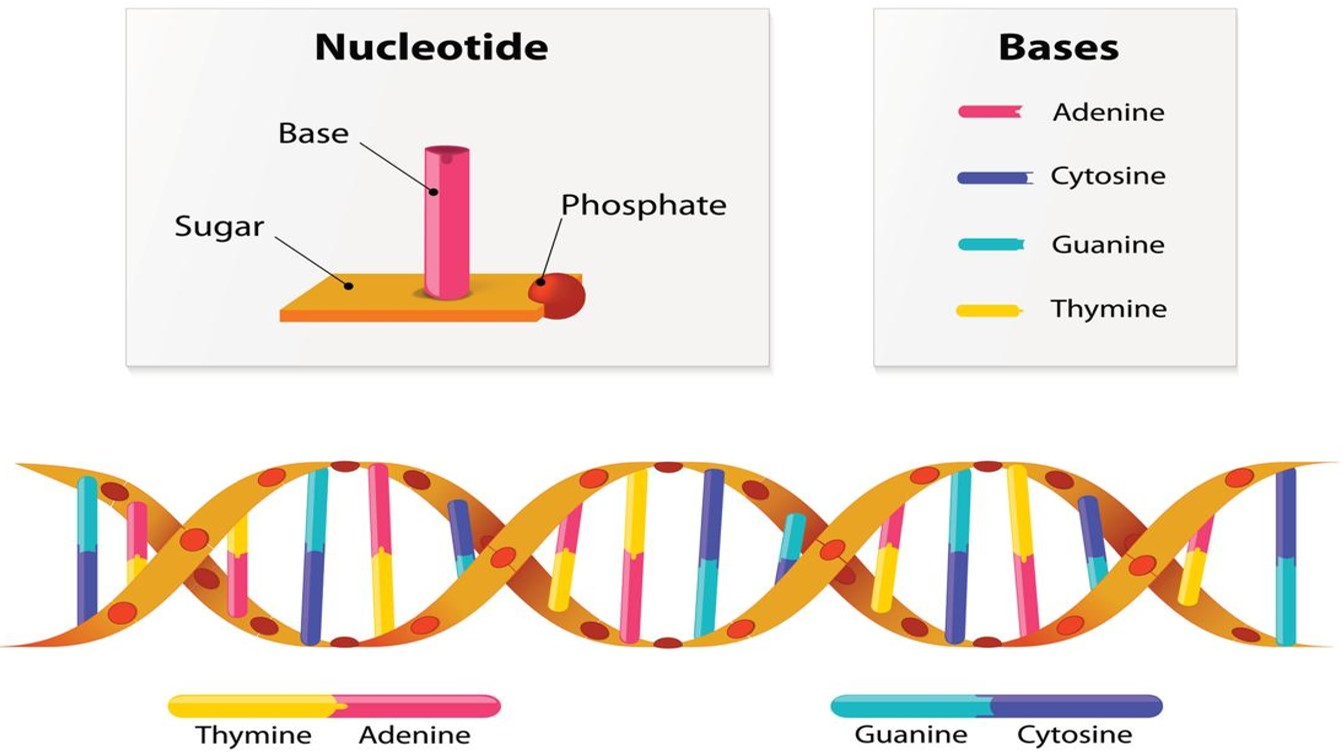
\includegraphics[width=\linewidth]{DNAStructure.jpg}
 	\caption{La struttura del DNA e del nucleotide.}
  	\label{fig:DnaAndNucleotideStructure}
\end{figure}
\newline
La struttura è caratterizzata da una doppia elica di lunghezza variabile, dove ciascun filamento è formato da una sequenza di molecole chiamate \textit{desossiribonucleotidi}.
\newline
Un desossiribonucleotide è composto da una molecola di zucchero, un gruppo fosfato ed una base azotata. Di quest'ultima, ne esistono quattro tipi:
\begin{itemize}
	\item \textit{adenina} (A);
	\item \textit{timina} (T);
	\item \textit{guanina} (G);
	\item \textit{citosina} (C).
\end{itemize}
Una proprietà importante delle basi azotate è che sono biunivocamente legate tra loro: l'Adenina si può legare solo con la Timina (A-T), mentre la Guanina con la Citosina (G-C). Questo significa che i filamenti sono complementari e quindi se conosciamo la sequenza di basi di un filamento di DNA sappiamo anche la sequenza di quello complementare.

\section{RNA}
L'\textit{RNA}, ovvero \textit{acido ribonucleico}, è una macromolecola caratterizzata da una struttura a singolo filamento composta da una sequenza di lunghezza variabile di \textit{ribonucleotidi}.
\newline
I ribonucleotidi si differenziano rispetto ai desossiribonucleotidi per una diversa molecola di zucchero e per la presenza della base azotata Uracile (U) che sostituisce la Timina.
\newline
Un tipo di RNA importante è l'\textit{RNA messaggero} (mRNA), che trasporta l'informazione genetica contenuta nel DNA in una regione cellulare (citoplasma) in cui avviene la sintesi delle proteine\footnote{La sintesi proteica è il processo attraverso il quale vengono prodotte nuove proteine.}.

\section{Proteine}
Le proteine sono le fondamenta di un organismo, infatti determinano la struttura e le funzioni delle cellule, ad esempio le cellule del cervello differiscono da quelle dei muscoli principalmente perché usano tipi diversi di proteine.
La loro struttura è composta da sequenze di \textit{aminoacidi} legati tra loro.
\newline
Sebbene esistano oltre cinquecento aminoacidi in natura, solo venti sono codificati dal codice genetico umano e pertanto utilizzati per la sintesi proteica.
\newline
La conversione dell'informazione genetica dal DNA in proteina, avviene in due processi, di seguito elencati:
\begin{enumerate}
	\item \textit{trascrizione}: viene prodotto l'RNA messaggero che trasporta l\?informazione nel citoplasma dove avverrà la traduzione;
	\item \textit{traduzione}: l'informazione contenuta all'interno del mRNA viene convertita in proteine.
\end{enumerate}